\documentclass[times, utf8, diplomski]{fer}

\usepackage{booktabs}
\usepackage{tikz}
\usepackage{indentfirst}
\usepackage{pgfplots}
\usepackage{graphicx}
\usepackage{caption}
\usepackage{subcaption}
\usepackage{graphicx}

\usetikzlibrary{matrix,calc}

\begin{document}

\thesisnumber{1382}
\title{Image Based Phylogenetic Classification}
\author{Vinko Kodžoman}

\maketitle

% Ispis stranice s napomenom o umetanju izvornika rada. Uklonite naredbu \izvornik ako želite izbaciti tu stranicu.
\izvornik

% Dodavanje zahvale ili prazne stranice. Ako ne želite dodati zahvalu, naredbu ostavite radi prazne stranice.
\zahvala{Thank you...}

\tableofcontents

\chapter{Introduction}
Since the dawn of time, people have tried to explain their surroundings. Life is all around us in many forms, and as such people have tried to categorize it by keen observation, both through its visual and genetic features. Today, it is organised into a taxonomic hierarchy of eight major taxonomic ranks. The number of known species on Earth is in the millions and climbing every year. Great numbers of species make it difficult to classify them only based on images and often requires domain knowledge. Therefore, an algorithm with the capability to classify species on the filed or from an image using only the image itself could provide great benefits for field researches.

Machine learning allows computers the ability to learn without being explicitly programmed \citep{samuel_studies_1959}. It, together with an increase in available quality data (CIFAR, Imagenet, Kaggle) has yielded great results in the area of deep learning - a class of machine learning algorithms. Deep learning algorithm's accuracy scales with the amount of data used by the algorithm, that together with the improvements in hardware - mainly general purpose graphic units (GPUs) - has yielded significant performance gains in the last couple of years. One of the most rapidly advancing filed of deep learning is image recognition \citep{krizhevsky_imagenet_2012, simonyan_very_2014, szegedy_going_2015, he_deep_2016} with new neural network architectures being developed almost at a yearly basis. The performance of deep neural networks on image recognition has achieved results previously thought impossible.

In this thesis I propose a solution for a scalable classification of species from images, based on convolution neural networks and recent modern deep learning techniques.

\chapter{Research context}
To fully understand the depth of the image recognition using deep learning, we need a better understand of the underlying algorithms and methods in machine learning, as well as fundamental terms and concepts. In the next section, an introduction of basic terms is given, followed by a detailed explanation of fundamental machine learning algorithms.

\section{Definitions and notation}

\subsection{Image representation}
Matrix is a rectangular array of numbers. It is used because some numbers are naturally represented as matrices. Matrix $A$ with $m$ rows and $n$ columns often written as $m \times n$ has $m*n$ elements and is denoted as $A_{m,n}$. Elements are denoted as $a_{i,j}$ where $i$ and $j$ correspond to the row and column number respectively, as shown in \ref{eq_2d_matrix}. 

\begin{equation} \label{eq_2d_matrix}
A_{m,n} = 
 \begin{bmatrix}
  a_{1,1} & a_{1,2} & \cdots & a_{1,n} \\
  a_{2,1} & a_{2,2} & \cdots & a_{2,n} \\
  \vdots  & \vdots  & \ddots & \vdots  \\
  a_{m,1} & a_{m,2} & \cdots & a_{m,n} 
 \end{bmatrix}
\end{equation}


Each image is represented as a 3 dimensional matrix. One pixel in the image represent a single element in the matrix and as images have multiple channels (RGB) each channel is a 2 dimensional matrix. Image $I$ denoted as $I_{k,m,n}$ where $k\in[0,2]$ represent the channel - red, green or blue - and $m,n\in[0,255]$ represent the pixel intensities in a particular channel as 2 dimensional matrices. Figure \ref{fig:image_matrix} shows a representation of an image as a 3 dimensional matrix where each pixel is denote as $I_{k,m,n}$.


\begin{figure}
\centering
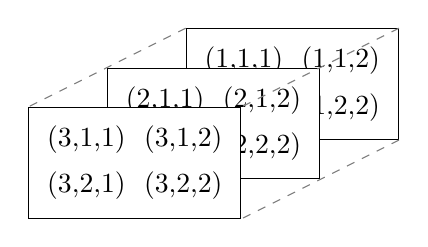
\begin{tikzpicture}
\def\xs{1} %shift in x direction
\def\ys{0.5} %shift in y direction
\def\nm{3} % number of 2d matrices in the 3d matrix
\foreach \x in {1,2,...,\nm}
{

\matrix [draw, % for the rectangle border
         fill=white, % so that it is not transparent
         ampersand replacement=\&] %see explanation
(mm\x)%give the matrix a name
at(-\x * \xs, -\x * \ys) %shift the matrix
{
    \node {(\x,1,1)}; \& \node {(\x,1,2)};\\
    \node {(\x,2,1)}; \& \node {(\x,2,2)};\\
};
}

\draw [dashed,gray](mm1.north west) -- (mm\nm.north west);
\draw [dashed,gray](mm1.north east) -- (mm\nm.north east);
\draw [dashed,gray](mm1.south east) -- (mm\nm.south east);
\end{tikzpicture}
\caption{RGB image with 4 pixels  represented as a 3 dimensional matrix}
\label{fig:image_matrix}
\end{figure}

\subsection{Gradient}
\label{se:gradient}
A gradient is a generalization of the derivative in multi-variable space and as such it is represented as a vector. Like the derivative, it represents the slope of the tangent of the graph of the function. Therefore, it points in the direction of the greatest rate of increase of the function. Gradients are widely used in optimization theory as they allow the parameters to shift in a direction which will minimize or maximize a given function. In machine learning the function we want to minimize will be the loss function, which we will define in further chapters in more detail. Gradient of $f$ is denoted as $\nabla{f}$, where every component of $\nabla{f}$ is a partial derivative of $f$, denoted as $\frac{\partial{f}}{\partial{x}}\vec{e}$. Notice that gradient components are vectors denoted as $\vec{e}$. Every vector is written with an horizontal arrow above the letter - $\vec{a}$. The gradient for a $n$ dimensional space is defined in \ref{eq:gradient}.


\begin{equation} \label{eq:gradient}
    \nabla{f}= \frac{\partial{f}}{\partial{x_{1}}}\vec{e_1} + \hdots + 	   \frac{\partial{f}}{\partial{x_{n}}}\vec{e_n}
\end{equation}

\subsection{Activation functions} \label{se:activation_functions}
Machine learning models use nonlinear functions to gain more capacity - expressiveness
. The most popular nonlinear functions are $sigmoid$, $tanh$, $relu$. All nonlinear functions have to have easy to compute gradients, as they are computed on parameters in order to reduce loss as explained above. 
\begin{equation} \label{eq:sigmoid}
	sigmoid(x) = \frac{1}{1 + e^{-x}}
\end{equation}

\begin{equation} \label{eq:tanh}
	tanh(x) = \frac{1 - e^{-2x}}{1 + e^{-2}}
\end{equation}

\begin{equation} \label{eq:relu}
	relu(x) = max(0, x)
\end{equation}
The order of nonlinear functions is given in order of their discoveries. Today relu is used the most, since it solves the problem of vanishing gradients for very deep neural networks, this does not apply to all network types. Recurrent neural networks (RNN) are a class of neural networks that often use $tanh$ as it is better suited for the particular recurrent architecture.

\begin{figure}
    \begin{subfigure}[b]{0.32\textwidth}
        \centering
        \resizebox{\linewidth}{!}{
            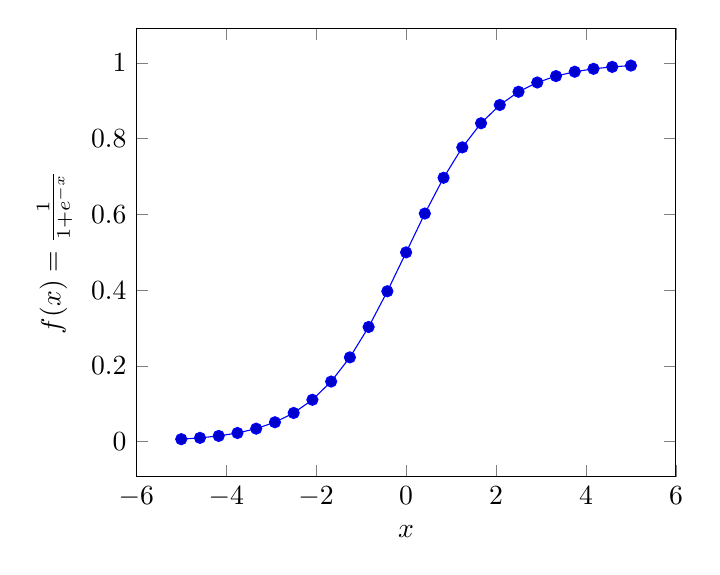
\begin{tikzpicture}
  			\begin{axis}[ 
	  			mark=none,
    			xlabel=$x$,
		    	ylabel={$f(x) = \frac{1}{1 + e^{-x}}$}
		    	] 
	   	 	\addplot {1 /(1 + e^-x)}; 
  			\end{axis}
            \end{tikzpicture}
        }
        \caption{$simgoid$}
        \label{fig:sigmoid}
    \end{subfigure}
    \begin{subfigure}[b]{0.32\textwidth}
    \centering
        \resizebox{\linewidth}{!}{
            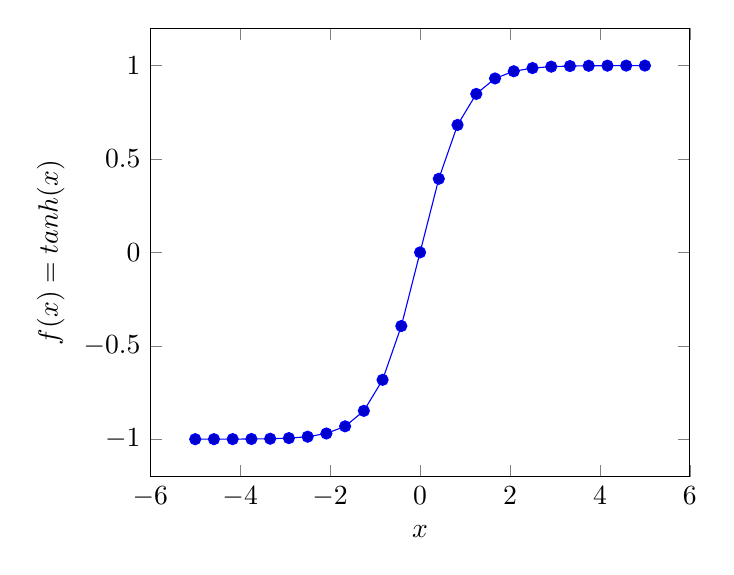
\begin{tikzpicture}
  			\begin{axis}[ 
	  			mark=none,
    			xlabel=$x$,
		    	ylabel={$f(x) = tanh(x)$}
		    	] 
	   	 	\addplot {tanh(x)}; 
  			\end{axis}
            \end{tikzpicture}
        }
        \caption{$tanh$}   
        \label{fig:tanh}
    \end{subfigure}
    \begin{subfigure}[b]{0.32\textwidth}
        \centering
        \resizebox{\linewidth}{!}{
            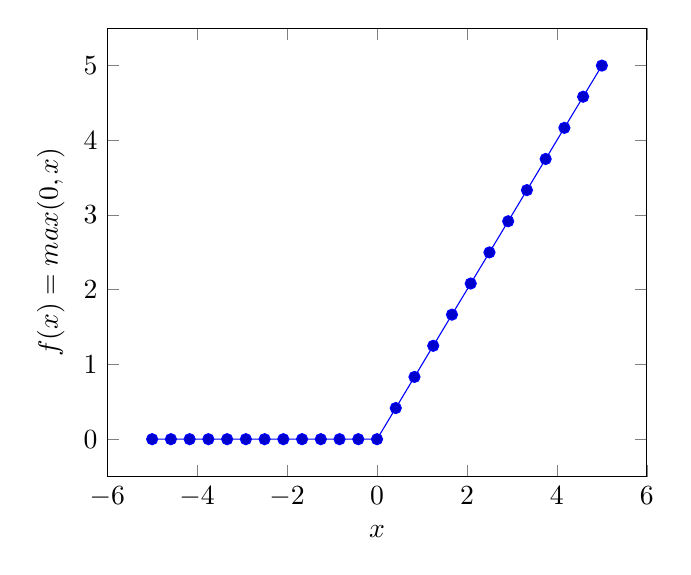
\begin{tikzpicture}
  			\begin{axis}[
  				mark=none,
    			xlabel=$x$,
		    	ylabel={$f(x) = max(0, x)$}
		    	] 
	   	 	\addplot {max(0,x)}; 
  			\end{axis}
            \end{tikzpicture}
        }
        \caption{$relu$}
        \label{fig:relu}
    \end{subfigure}
\caption{Nonliear activation functions} 
\label{fig:subfig1.a.4}
\end{figure}

\subsection{Metrics}
In order to compare different models a set of metrics is employed. Accuracy which gives the accuracy of a model, it is often used on balance datasets (\ref{eq:accuracy}). The problem with unbalanced datasets can be easily explained with a short example. Image having $2$ classes $K=\{dog,cat\}$ and there are a total of $100$ images in the dataset, of which only $2$ are dogs. The model if optimized for accuracy might say the whole dataset is cats which will yield an accuracy of $98\%$. To solve the previous problem, additional metrics were introduced for the task of classification; precision (\ref{eq:precision}), recall (\ref{eq:recall}) and F1 score (\ref{eq:f1score}). Precision - positive predictive value - is defined as a fraction of retrieved instances that are relevant. Recall - sensitivity - is a fraction of relevant instances that are retrieved. In order to represent the performance of a model as a single variable F1 score was introduced, it represent a harmonic mean of recall and precision.
\begin{equation} \label{eq:accuracy}
	Accuracy = \frac{tp + tn}{tp + tn + fp + fn}
\end{equation}

\begin{equation} \label{eq:precision}
	Precision = \frac{tp}{tp + fp}
\end{equation}

\begin{equation} \label{eq:recall}
	Recall = \frac{tp}{tp + fn}
\end{equation}

\begin{equation} \label{eq:f1score}
	F1 score = 2 * \frac{precision * recall}{precision + recall}
\end{equation}



Classification results are often represented as a confusion matrix, also known as an error matrix.  It is a performance visualisation of a classification model - classifier. To build the classification matrix, conditions of the experiment must be labelled as positive and negative. Using the cats and dogs example from before and marking the cats and a positive and dogs as a negative class. Doing so creates a $2x2$ matrix of actual and predicted values as shown in table \ref{tb:confusion_matrix}.

\begin{table}
\centering
\caption{Confusion matrix}
\label{tb:confusion_matrix}
\begin{tabular}{|c|c|c|}
\hline 
 & \textbf{prediciton} positive & \textbf{prediction} negative \\ 
\hline 
\textbf{actual} positive & True Positive (TP) & False Positive (FP) \\ 
\hline 
\textbf{actual} negative & False Negative (FN) & True Negative (TN) \\ 
\hline 
\end{tabular}
\end{table}

\subsection{Data} \label{se:data}
The input data of the machine learning algorithm is labelled as $D$, and it consists of $X$ and $y_{t}$, where $X$ is one input data point (an image in our case) and $y_{t}$ is the true label of the picture - species' name. Written formally the whole input dataset is represented as $D = \{{X}^{\,i},y^{\,i}\}^{N}_{i=1}$, where $i$ is the $i$-th data point and $N$ in the number of data points. Prediction of the algorithm is labelled as $y_{p}$.

The input data set is usually split into two datasets called the \textit{training} a \textit{test} dataset. The training dataset is used to optimize them models parameters while the test data is used to evaluate the model's performance. Sometimes the training dataset is split further into training and \textit{validation} where the validation dataset is used to tune the models \textit{hyperparameters}. Hyperparameters are parameters that do not belong to the model but non the less effect the model's performance. Depth of the neural network is a hyperparameter and will be discussed in later chapters in more detail.


\section{Machine learning}
\label{se:machine_learning}

As said in the Introduction chapter, machine learning allows computers the ability to learn. Giving data to a machine learning algorithm - model - allows it to find patterns within the dataset. The function that maps the input $X$ to $y_p$ is called a \textit{hypotesis} and is denoted as $h$ (\ref{eq:hypotesis}). The hypotesis $h(X ; \vec{\theta})$ is parametrized with $\vec{\theta}$ - model's parameters.

\begin{equation} \label{eq:hypotesis}
	h(X ; \vec{\theta}) : X \to y
\end{equation}


The model is defined as a set of hypothesises $H$, $h \in H$. Machine learning is the search of the best hypothesis $h$ from the hypothesis space $H$ - typical optimization problem. The algorithm tries to minimize the empirical error function $E(h|D)$ - loss function. The error indicates the accuracy of the hypothesis and is called empirical because it is computed on $D$. Therefore, every machine learning algorithm is defined with the model (\ref{eq:model}), error function (\ref{eq:error_function}) and the optimization method (\ref{eq:optimization_function}).

\begin{equation} \label{eq:model}
	H = \{ h(X ; \vec{\theta}) \}_{\theta}
\end{equation}

\begin{equation} \label{eq:error_function}
	E(h|D) =  \frac{1}{N} \displaystyle\sum_{i=1}^{N} I\{h(X^{\,i}) \neq y^{i}\}
\end{equation}

\begin{equation} \label{eq:optimization_function}
	\theta^{*} = argmin_{\theta} E(\theta | D)
\end{equation}


Machine learning algorithms are divided into groups depending on the task, the groups are classification and regression. Each can be represented as a result of $h(X ; \vec{\theta})$. Classification hypothesis takes the input $X$ and returns a class $k$, example of this method would be image classification. Regression hypothesis takes the input $X$ and returns a number, for example predicting house prices.

\begin{equation} \label{eq:regression_def}
	Regression \equiv h(X ; \vec{\theta}) : X \to y, y \in \mathbb{R}
\end{equation}

\begin{equation} \label{eq:classification_def}
	Classificatio  \equiv h(X ; \vec{\theta}) : X \to y, y \in K = \{k_{0}, ..., k_{n}\}
\end{equation}

In this chapter we mentioned that machine learning algorithms are trained by minimizing the empirical loss, and in the subsection \ref{se:data} we mentioned the idea of having a training and test set. The goal of the machine learning model is to have good generalization - the ability to perform well on never before seen data $X$. The training set $X_{train}$ is used by the optimization algorithm to tune the model's parameters, while the test set $X_{test}$ is used to evaluate the generalization performance of the model. If the optimization algorithm does not know when to stop it can learn the whole training set and be able to predict every value, this is called overfitting and it is to be avoided. When the model overfits, it learns to predict based on the data points in $X_{train}$ instead of the learning the underlying patterns in $X_{train}$, which in turn leads to poor generalization performance. This is commonly seen in models with high capacity. On the other hand, if the model has low capacity, it will under-perform - work below its potential. That is referred to as underfitting. To goal is to find the optimal spot of the model's performance - between underfitting and overfitting. This behaver can be seen in figure \ref{fig:overfitting}. The x-axis shows the number of training epochs - each epoch increases the capacity of the model. We see that the training error $E_{train}$ is falling asymptotically towards zero while the the generalization performance start to fall certain a point (50 epochs). The ideal situation for the model is to stop the training when the model starts to overfit, which is not that easy as we will see in the future chapters.


\begin{figure}
  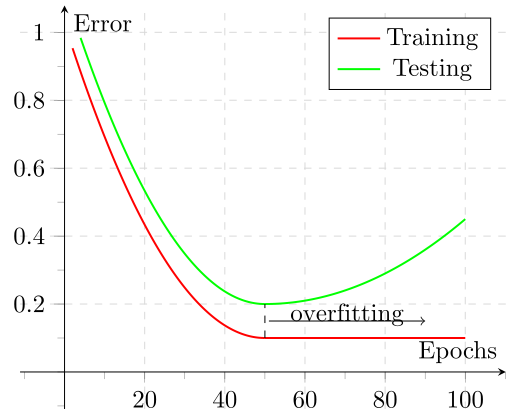
\includegraphics[width=0.8\textwidth]{figures/overfitting.png}
  \centering
  \caption{Performance of a model with time using training and test set}
  \label{fig:overfitting}
\end{figure}



One way to combat overfitting is by early stopping during training. Another, more popular way is to use regularization. Regularization is a technique for increasing the generalization performance of the model. There is a broad set of regularization techniques used in machine learning models. Some of the most popular for artificial neural networks are called dropout \citep{srivastava_dropout:_2014} and data augmentation, both of which will be explained in more detail in future chapters (subsections \ref{se:dropout} and \ref{se:data_augmentation}). Regularization techniques usually add additional components to the loss function in order to prevent the model from learning to map $X_{train}$ to $y_{train}$ directly.


\subsection{Supervised and unsupervised learning}
For the model to be train it needs data $D$ which is defined as $\{{X}^{\,i},y^{\,i}\}^{N}_{i=1}$. Unfortunately, $y$ is not always available. In such cases, the model can still use only $X$ to infer and that is called unsupervised learning. When the model uses both the data points $X$ and labels $y$ it is called supervised learning. Classification and regression are both cases of supervised learning. Cluster analysis or more commonly called clustering is a type of unsupervised learning. In clustering the model tries to group a set of objects in such a way that objects in the same group are more similar based on a cretin metric. The groups are called clusters. Some algorithms need the number of clusters to be predefined, while others discern it by themselves. As the topic of this thesis is classification, in following chapters supervised learning methods will be explained in more detail.

\subsection{Artificial neural network (ANN)}
One of the most interesting models in machine learning, with a diverse set of variations are artificial neural network (ANN). The computational model based on mathematics for neural networks was first introduced in 1943 by Warren McCulloch and Walter Pitts \citep{mcculloch_logical_1943}  called threshold logic. Later on in 1951 a influential paper was published by S. C. Kleene on linking neural networks to finite state automata \citep{kleene_representation_1951}. Artificial neural networks are based on a large collection of small computational unites called neurons (figure  \ref{fig:ann_neuron}). The architecture was inspired by axons (\ref{fig:neuron}) from our biological brains. The idea is that even though a single neuron dose not have the capacity to express complicated levels of abstractions - neurons together can. Neurons are connect in order to transfer signals. If a neuron receives a strong enough signal it becomes activated and propagates the received signal toward his output. Just propagating the signal would not be of benefits, as the single would not transform while passing trough the network, therefore non linear activation functions, as explained in subsection \ref{se:activation_functions}, are added to each output of a neuron.

\begin{figure}
  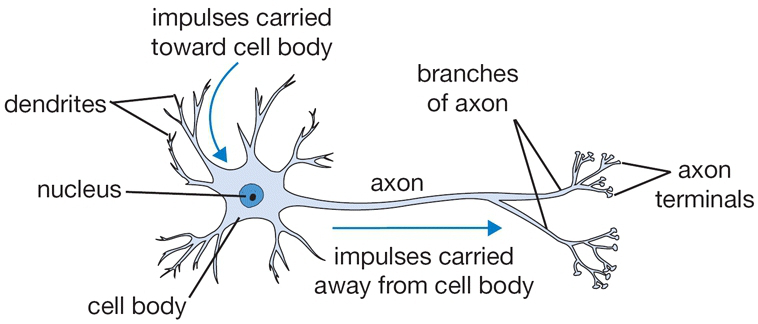
\includegraphics[width=\linewidth]{figures/axon.png}
  \caption{Neuron cell in a biological brain.}
  \label{fig:neuron}
\end{figure}

\begin{figure}
  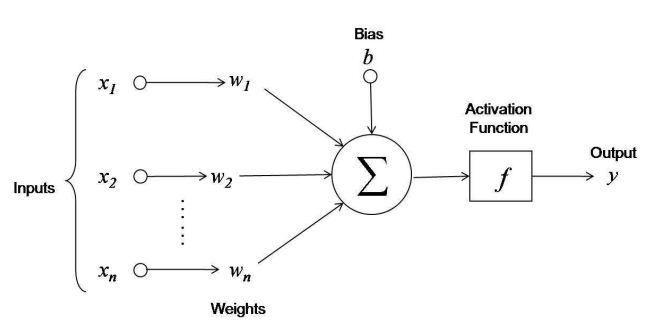
\includegraphics[width=\linewidth]{figures/neuron.jpg}
  \caption{Artificial neuron cell.}
  \label{fig:ann_neuron}
\end{figure}

One of the most popular ANN architectures are feed-forward networks (FFN), sometimes also referred to as fully-connected or dense. They are called feed-forward because the data $X$ enters at on side of the network (the input layer) and exits at the other end (output layer). Neurons are grouped into layers, and layers make an artificial neural network. The first layer is called an input layer, the last layer is called the output layer and everything in between are called hidden layers. The network is called fully-connected because each neuron in the hidden and output layers are connected with ever neuron of the previous layer as seen in figure \ref{fig:ann}.
Each neuron consists of connections, bias and activation function. Each connection has a weight that singles the importance of the connection to the neuron. To get the net output of the neuron we multiple the input vector $\vec{x}$ with the weight vector $\vec{w}$. As the bias (commonly denoted with $w_0$ or $b$), does not have an input of its own, we assigned $x_0$ to 1 so we can to a vector multiplication (\ref{eq:neuron_net_output}). To get the final output $y$ of the neuron, the activation function $f$ is applied to the $net$ output, as shown in \ref{eq:neuron_output}). computational model of the artificial neuron can bee seen in the figure \ref{fig:ann_neuron}.

\begin{equation}
	\label{eq:neuron_net_output}
	net = 1*w_0 + w_1*x_1 + ... + w_n*x_n = \vec{x} * \vec{w}
\end{equation}

\begin{equation}
	\label{eq:neuron_output}
	y = f(net) = f(\vec{x}*\vec{w})
\end{equation}

\begin{figure}
  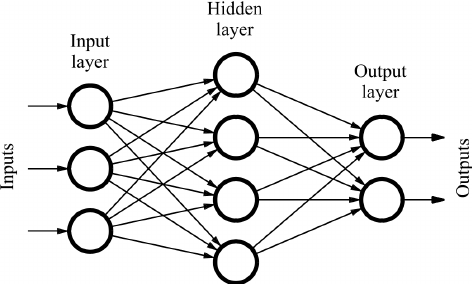
\includegraphics[width=\linewidth]{figures/ann.png}
  \caption{Feed-forward neural network}
  \label{fig:ann}
\end{figure}


Artificial neuron networks have the ability to adjust their capacity to the task. Adjusting the number of neurons in a single layer, the number of hidden layers or the type of activation function used in each neuron affects the capacity of the ANN. Such flexibility also leads to a broad number of architectures, and there is no clear way to determine which one suits best. It is often left to the user to test a broad variety of architectures. Looking at the figure \ref{fig:ann} we can see that the number of neurons in the input layer matches the input size, this is true also for the output layer. Therefore, when designing an ANN the size of input and output layers are determined by the task and the number of hidden layers by the user.


\section{Deep learning}
Deep learning is a class - subset - of machine learning algorithms. Even though, deep learning may be connect to using "deep" neural networks - neural networks with many layers - it was created as a subset of machine learning that promised the automation of feature extraction task by using unsupervised learning. Unsupervised feature extraction and feature representation is done through a cascade of many nonlinear layers, each of which contains artificial neurons. 

Visual recognition is one of the fields that is most affected by improvements in deep learning. It's difficult and time consuming to build hand crafted features for each visual recognition problem. Deep learning allows the user to use raw images without any preprocessing - making it applicable with ease to almost any task.

Deep learning algorithms consist of enormous numbers of  artificial neurons (hundreds of millions), therefore training them is computational expensive. Recent breakthroughs in deep learning were driven by advances in hardware - graphics processing unit (GPUs). GPUs are made of a lot of processor unites, making them ideal for highly concurrent tasks. Neural networks are easily trained concurrently because of their composite structure and a special training algorithm called stochastic backpropagation (discussed in detail in subsection \ref{se:backprop}), commonly referred to as backprop.

\subsection{Convolutional Neural Network (CNN /  ConvNet)}
Convolutional neural network is a type of feed-forward network that was inspired by the organization of animal's visual cortex. They are used in recommender systems, natural language processing and image recognition. The architecture was inspired by the works of Huble and Wiesel in 1950s and 60s \citep{hubel_receptive_1968}, their work showed that animal's visual cortex contains neurons that individually responds to small regions in the visual field. Their experiments showed that neighbourhood neurons had similar receptive fields.

The necognitron was introduced in 1980s by Kunihiko Fukushima \citep{fukushima_neocognitron:_1982, eckmiller_hierarchical_1989} and served as an inspiration for today's modern convolutional neural network architecture. The necognitron is a hierarchical multilayered artificial neuron network. It was used for handwritten character recognition, which belongs in the domain of image recognition.

\begin{figure}
  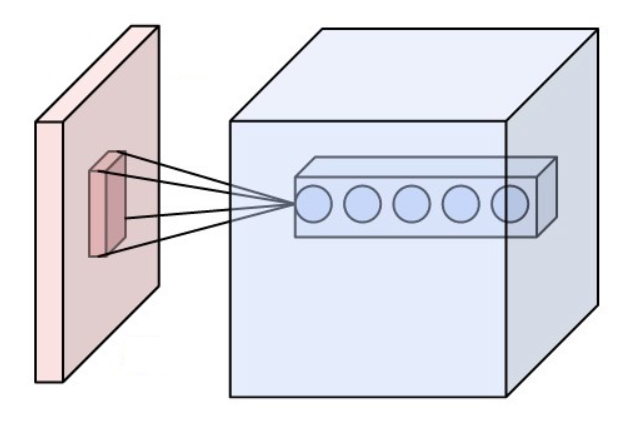
\includegraphics[scale=0.5]{figures/conv.png}
  \centering
  \caption{3D structure of a convolutional filter (on the left painted in pink is the input and the blue rectangle with circle is a filter)}
  \label{fig:conv}
\end{figure}

Today's modern convolutional neural network architectures, such as: AlexNet, VGG, Inception and ResNet \citep{krizhevsky_imagenet_2012, simonyan_very_2014, szegedy_going_2015, he_deep_2016} are made mostly of convolution and pooling layers. These architecture have an enormous number of parameters and are trained on powerful GPUs or clusters of servers over a period of days, sometimes even weeks.

The convolution layer is a building block of modern CNNs. The layer's parameters consist of a set of kernels (filters). Each filter has a small receptive field, but extends through the whole depth of the input. During the forward pass of the input through the network, each filter is convolved across the width and heigh of the input volume. Each time the filter moves to neighbourhood pixels it creates an output pixel (shown in figures \ref{fig:conv} and \ref{fig:conv1}). Each convolutional layer consists of multiple filters, each specialized (because of training) to detect different features in the input. Filters will detect diagonal edges, top edges, corners, etc. Each filter will use the features of the previous layer to create more abstract features. For example, a filter in the first layer might capture edges, while filters in deeper layers may use the edge filters to create corner and circle detectors (shown in detail in figure \ref{fig:filter}) \citep{simonyan_very_2014}.


\begin{figure}
  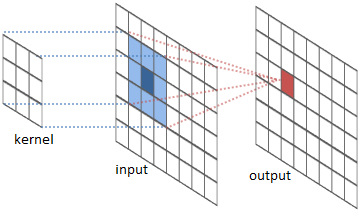
\includegraphics{figures/conv1.png}
  \centering
  \caption{A 3x3 kernel (filter) convolving and input to generate an output}
  \label{fig:conv1}
\end{figure}

\begin{figure}
  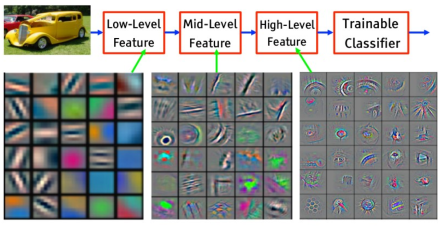
\includegraphics[scale=1.4]{figures/filter.png}
  \centering
  \caption{Representation of filters through the CNN}
  \label{fig:filter}
\end{figure}

The second core layer of almost every modern CNN is the pooling layer. It, in contrast to the convolution layer, does not have any parameters. Pooling layer takes the input and reduces its dimension. CNNs use max pooling, which maps the input into a reduced output by taking only the max values in the mapping (showed in figure \ref{fig:pool}). Use of pooling layer is a heated topic in today's CNN architectures, unfortunately hardware can't keep up with the depth of the modern architectures without the use of pooling layers.

\begin{figure}
  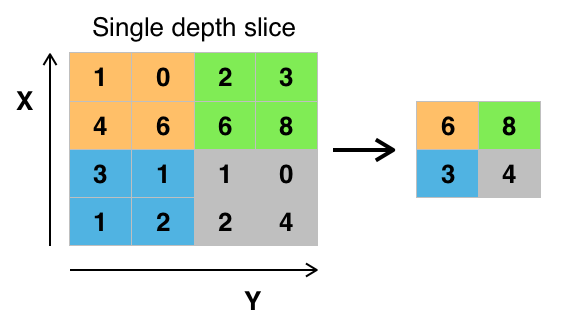
\includegraphics[scale=0.6]{figures/pool.png}
  \centering
  \caption{Max pooling a 4x4 input to 2x2}
  \label{fig:pool}
\end{figure}

The typical structure in a CNN network will be a couple of convolution layers followed by a max pool layer. The most common dimension of convolution filters is 3x3, made popular by the huge success of VGG \citep{simonyan_very_2014}. The typical CNN is shown in figure \ref{fig:cnn}.

\begin{figure}
  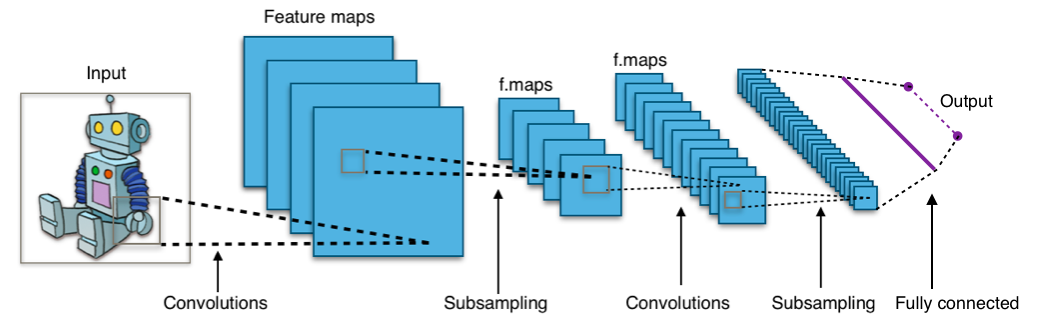
\includegraphics[scale=0.43]{figures/cnn.png}
  \centering
  \caption{Typical modern CNN}
  \label{fig:cnn}
\end{figure}

\subsection{Dropout} \label{se:dropout}

On of the most important techniques in machine learning is regularization (subsection \ref{se:machine_learning}). The modern approach to regularization is called dropout and was introduced in 2014 \citep{srivastava_dropout:_2014}. Dropout "drops" (removes) a percent of neurons on every forward pass (figure \ref{fig:dropout}). The network cannot count that the same neurons will always be active and, as a result it increases the robustest of the model together with its generalization performance. As in every forward pass, the network has a different set of neurons, this technique can be seen as using multiple variations of the same network on the same problem.

\begin{figure}
  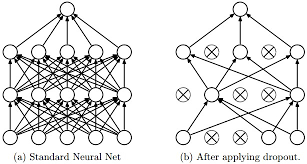
\includegraphics[scale=0.91]{figures/dropout.png}
  \centering
  \caption{An example of the dropout technique}
  \label{fig:dropout}
\end{figure}

\subsection{Data Augmentation}  \label{se:data_augmentation}

Another popular regularization technique is called data augmentation. The model usually trains in tens or even hundreds of epochs - a signal epoch is when the training algorithm uses every data point in $X_{train}$ (one pass over $X_{train}$). Reusing the same data points can lead to overfitting. To prevent that we can augment $X_{train}$ on every epoch. This approach is commonly called data jittering. Usually the data is augmented with rotation, mirroring, cropping, blurring (all these effects can be seen in figures \ref{fig:data_augmentation_figure} and \ref{fig:data_augmentation}). Both, dropout and data augmentation is used in almost every state-of-the-art CNN model today. There are some exceptions due to a new technique called batch normalization \citep{ioffe_batch_2015}.

\begin{figure}
  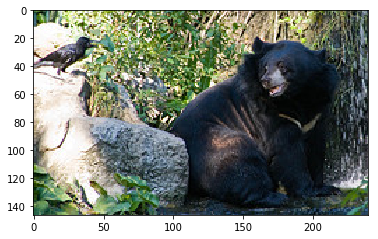
\includegraphics[scale=0.7]{figures/data_augmentation.png}
  \centering
  \caption{An example of the original image 224x224x3 in $X_{train}$}
  \label{fig:data_augmentation_figure}
\end{figure}

\begin{figure}
  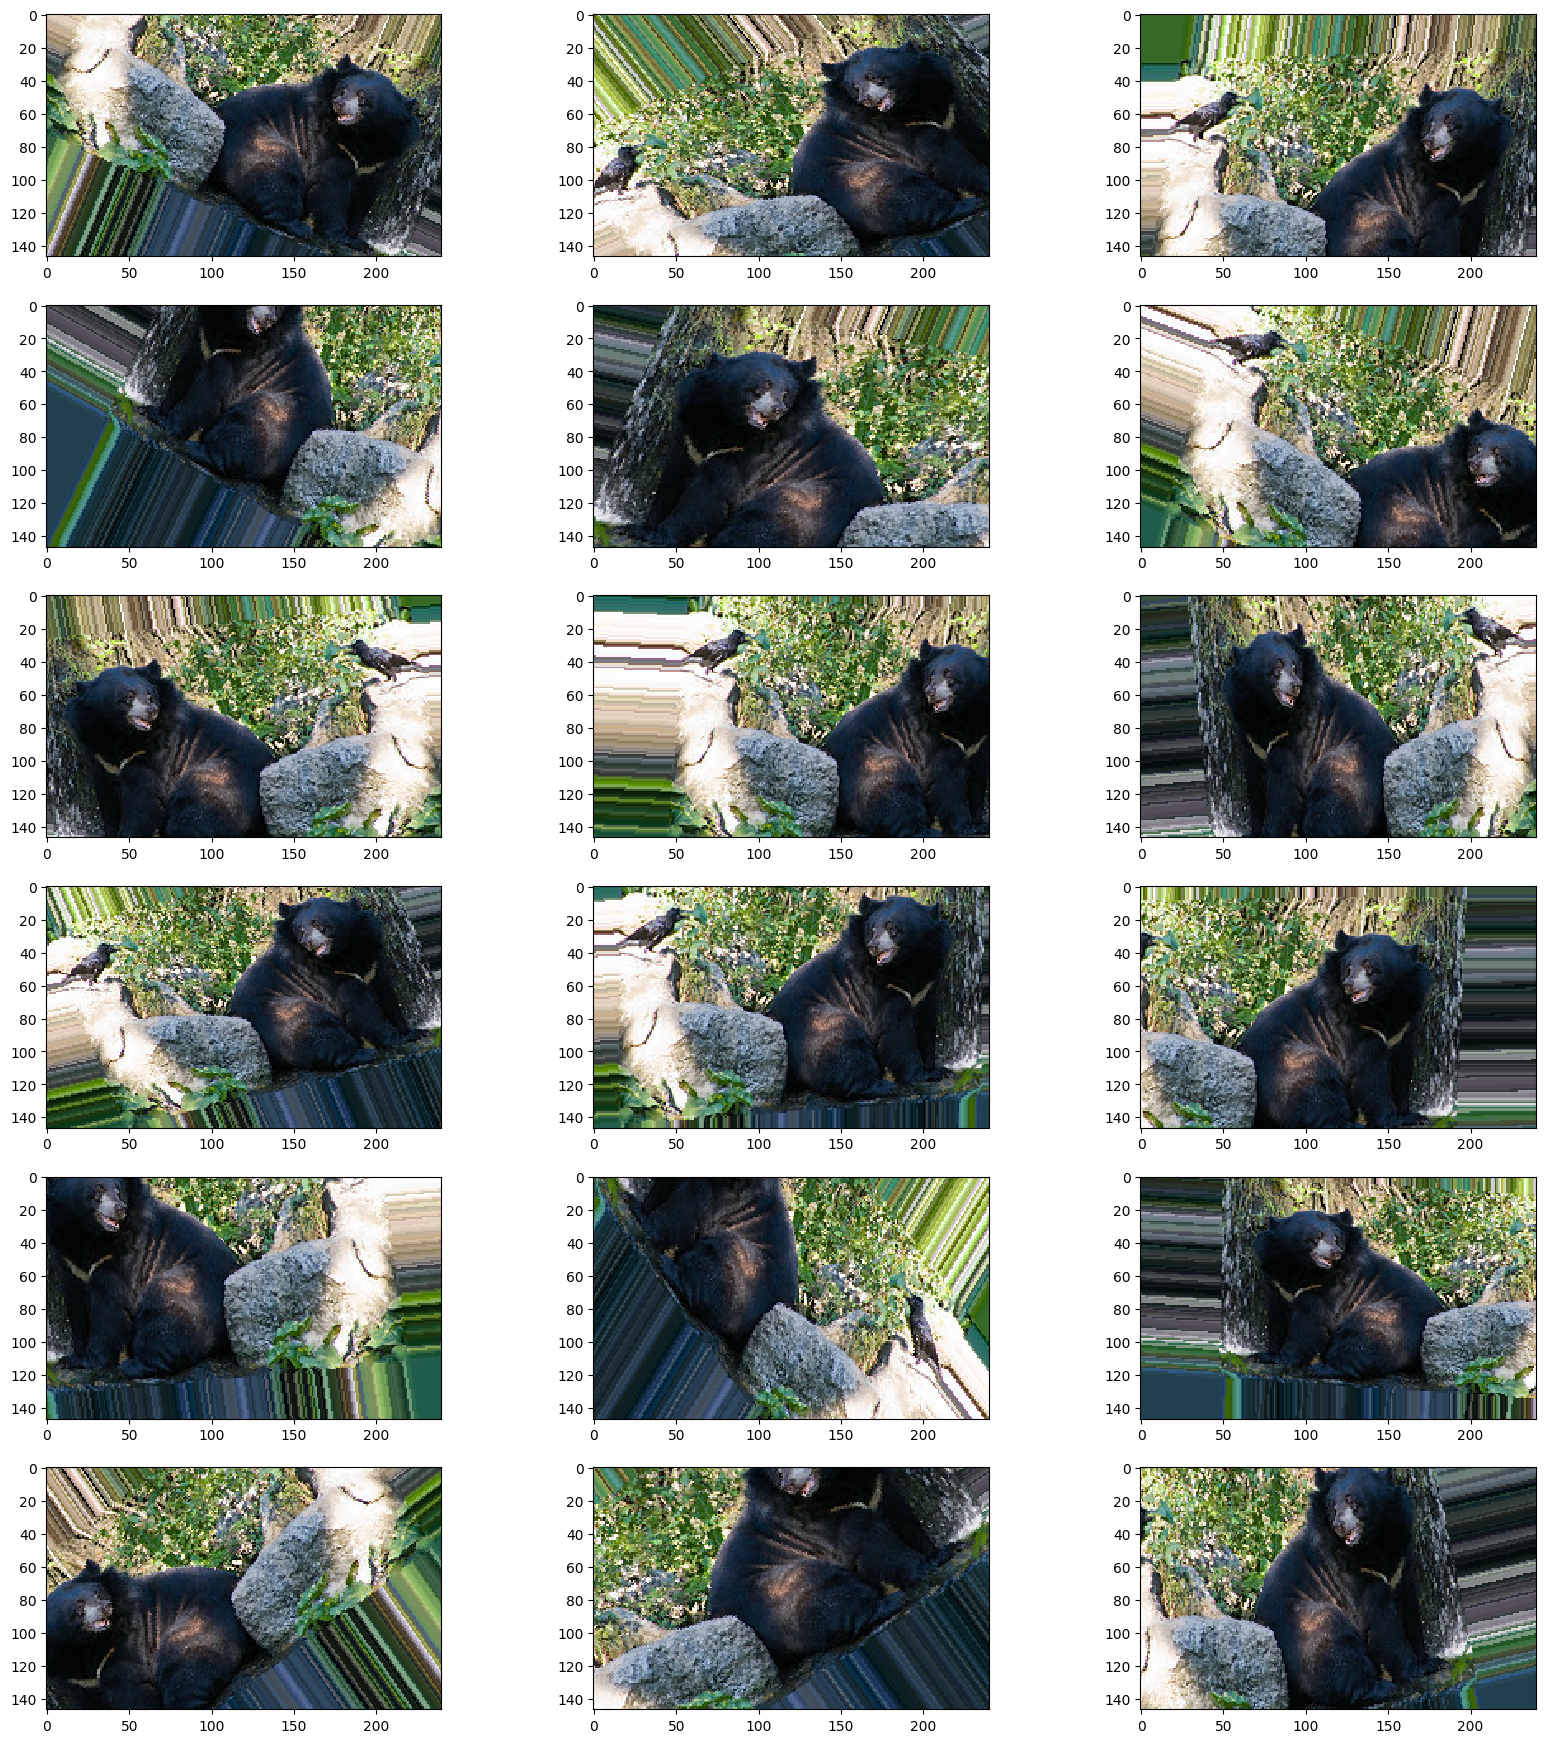
\includegraphics[scale=0.35]{figures/da1.png}
  \centering
  \caption{Example of data augmented images based on the original image \ref{fig:data_augmentation_figure}}
  \label{fig:data_augmentation}
\end{figure}

\subsection{Backpropagation} \label{se:backprop}

To be able to train the convolution neural network on huge datasets, we need an algorithm that allows us to train the model with a subset of $X_{train}$. Fitting the whole $X_{train}$ in the GPU memory is not possible for datasets of serious size. Also, the algorithm should be highly concurrent in order to use the structure of neural network to its advantage. The backward propagation of errors or more commonly called backpropagation (backprop) used together with gradient descent is the most popular method for training most neural networks.

\subsubsection{Gradient Descent}

Gradient descent is an iterative optimization algorithm. It uses the gradient \ref{se:gradient} of  a function find a point on a domain that minimises or maximises the function's value. Gradient descent does not guarantee to find the global maxima or minima (figure \ref{fig:local_and_global_function_values}). There have been several variations of the gradient descent algorithm that deal with the algorithm being stuck in local maxima, the most famous and most widely used at this moment is Adam \citep{kingma_adam:_2014}.

\begin{figure}
  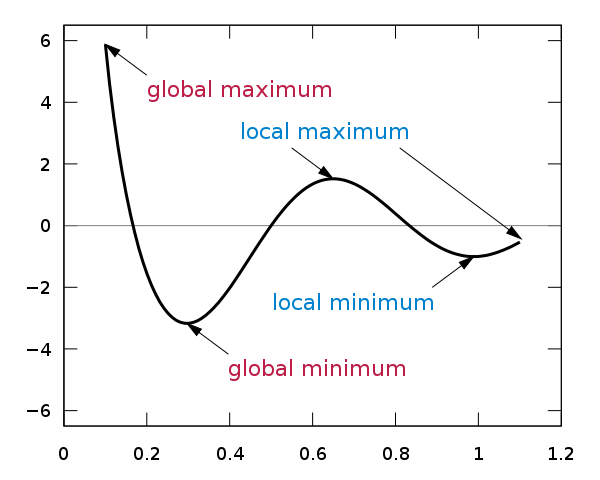
\includegraphics[scale=0.5]{figures/local_global_maxima_minima.png}
  \centering
  \caption{An example of local and global maxima and minima in a function}
  \label{fig:local_and_global_function_values}
\end{figure}

\begin{equation} 
\label{eq:gradient_descent}
	x_{n+1} = x_n - \eta * \nabla{f(x_n)}
\end{equation}

Gradient descent uses the gradient to move in a way that minimises or maximises the given function (\ref{eq:gradient_descent}). The amount that is used to move the data point - called the step ($\eta$) - is crucial for the convergence of the algorithm. If the step is too big the algorithm might diverge, while if the step is too small the algorithm might take too long to converge. Gradient descent, like many other optimization algorithms needs to have its parameters properly tuned.

\begin{figure}
  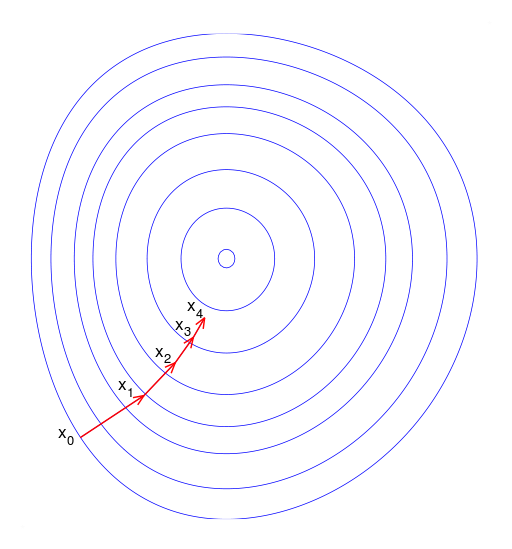
\includegraphics[scale=0.5]{figures/gradient_descent.png}
  \centering
  \caption{An example of gradient descent converging to global minima in a 2D space (2 variable function)}
  \label{fig:local_and_global_function_values}
\end{figure}

\subsubsection{Stochastic Gradient Descent}

The main disadvantage of the gradient descent (\ref{eq:gradient_descent}) is the need to calculate the gradient on all the dataset for the update state. The gradient has to be calculate on the whole $X_{train}$. A huge improvement on the basic gradient descent is a the stochastic gradient descent. It updates the gradient by sampling the dataset in a minibatch, usually the size 64, 128 or 256 data points (depending on GPU memory limitations). After every epoch the the whole training dataset $X_{train}$ is shuffled so that different minibatches will be sampled. The rule of thumb is if you can increase the size of minibatch - do it. The more data points are in the minibatch, the more precise is the gradient approximation, also the model trains faster.

\subsubsection{Optimization Target}

The goal of the gradient descent algorithm is to minimise or maximise a function. In deep learning, when training the model, we want to minimise the loss function $E(h|D)$ by computing its gradient. In classification (\ref{eq:classification_def}) the goal is to predict for the predicted class $y_p$ to match the true class $y_t$. Neural networks for classification usually have a softmax layer as their last layer. Softmax (\ref{eq:softmax}) is a normalization exponential function, which transforms neural network's outputs to probabilities for every class. The sum of the softmax values for all classes is equal to 1.  

\begin{equation}
\label{eq:softmax}
	softmax(\vec{z})_j = \frac{e^{z_j}}{\displaystyle\sum_{k=1}^{K} e^{z}_k} \quad \text{for} \quad j = 1, ..., K
\end{equation} 

For the task of classification, the softmax function is the final layer - the output. Using this information allows us to compute the loss function. The loss of a softmax function is called cross-entropy loss and is computed with negative log likelihood (\ref{eq:cross_entropy_loss}).

\begin{equation}
\label{eq:cross_entropy_loss}
	L(y_t, y_p) = - \displaystyle\sum_{d=1}^{D} \sum_{k=1}^{K} y^i_t * log(y^i_p) 
\end{equation}

To use the cross-entropy loss in the backpropagation we have to calculate its gradient. The gradient for cross-entropy loss is shown in \ref{eq:cross_entropy_graidnet}).

\begin{equation}
\label{eq:cross_entropy_graidnet}
 \nabla{L} = \vec{y_t} - \vec{y_p}
\end{equation}

\subsection{Vanishing Gradient}
\label{se:vanishing_gradient}

On of the problems in using backpropagation is the propagation of loss gradients in the neural networks. As the neural network is composed of smaller unites called neurons, its output is also a function composed of linear combinations and non-linear activation functions of previous layers. The backpropagation algorithm calculates the gradient losses from the output to the front layers of the neural network - hence the name backpropagation. The deeper the network, the more information is lost duo to gradient decay - low gradient values. The vanished gradient means that the network is not efficiently training and leads to poor performance. One way to combat that is to use special activation functions \citep{clevert_fast_2015, xu_empirical_2015, he_delving_2015} or special architectures \citep{he_deep_2016}. 



\subsection{Batch Normalization}
\label{se:batch_norm}

Normalizing input data before it enters the machine learning algorithm usually increases the performance of the algorithm. It is easier for the model to learn that all of its inputs will be in a certain range. Input normalization in neural networks will not yield significant performance improvements because the input for images are normalized by nature in the range of $1$ to $255$ RGB (\ref{se:data}). The second problem is the modularity of neural networks. Each layer feeds its outputs into the inputs of the next layer - making any input normalization futile. To combat this a new solution in a form of normalization layer has been introduced in 2015 called batch normalization \citep{ioffe_batch_2015}. It normalizes the data for the whole batch that is used in the forward pass of the backpropagation algorithm (\ref{se:backprop}). As the authors have showed, using batch normalization improves generalization, in some cases removes the need for dropout (\ref{se:dropout}) and makes the neural network more robust to initial hyperparameter initialization.

\chapter{TaxNet}
To make a scalable species classifier that works with specific hardware requirements I had to make a classifier that yields the best performance and could be trained on a GPU with 2GB of VRAM in a reasonable time frame. In this chapter I introduce my solution - the TaxNet.


\section{Implementation}

\chapter{Dataset}
\subsection{ImageNet}

\chapter{Results}
Graphs graphs graphs...

\chapter{Conclusion}
Zaključak.

\bibliographystyle{fer}
\bibliography{master_thesis}


\begin{sazetak}
Sažetak na hrvatskom jeziku.

\kljucnerijeci{Ključne riječi, odvojene zarezima.}
\end{sazetak}

% TODO: Navedite naslov na engleskom jeziku.
\engtitle{Title}
\begin{abstract}
Abstract.

\keywords{Keywords.}
\end{abstract}

\end{document}